%%%%%%%%%%%%%%%%%%%%%%%%%%%%%%%%%%%%%%%%%%%%%%%%%%%%%%%%%%%%%%%%%
% Qualificacao de Doutorado / Dept Fisica, CFM, UFSC            %
% Andre@UFSC - 2013                                             %
%%%%%%%%%%%%%%%%%%%%%%%%%%%%%%%%%%%%%%%%%%%%%%%%%%%%%%%%%%%%%%%%%

%:::::::::::::::::::::::::::::::::::::::::::::::::::::::::::::::%
%                                                               %
%                          Capítulo 3                           %
%                                                               %
%:::::::::::::::::::::::::::::::::::::::::::::::::::::::::::::::%

%***************************************************************%
%                                                               %
%                        Decomposicao                           %
%                                                               %
%***************************************************************%

\chapter{Síntese de população estelar nas componentes morfológicas de galáxias}
\label{sec:Decomp}


%***************************************************************%
%                                                               %
%                    Decomposicao bojo-disco                    %
%                                                               %
%***************************************************************%

\section{Decomposição morfológica}
\label{sec:Decomp:decomp}
 
 % FIXME:
Uma forma de classificar as galáxias é pela sua morfologia. A mais conhecida é a
sequência de Hubble, onde galáxias são classificadas como elípticas ou
esferoidais, espirais, lenticulares ou de disco, e irregulares.
Neste trabalho trata-se apenas de galáxias com disco e esferoidais. Galáxias
esferoidais seguem em geral um perfil de Sérsic, conforme a equação
\begin{equation*}
I(r) = I_e \exp \left\{- b_n \left[ \left( \frac{a}{r_e} \right)^{\sfrac{1}{n}}
- 1 \right] \right\}.
\end{equation*}
Já galáxias de tipo disco são bem modeladas por um perfil exponencial, dado por
\begin{equation*}
I(r) = I_0 \exp \left(- r / h \right).
\end{equation*}

Uma galáxia pode ser bem descrita como a soma de um disco exponencial e um bojo
com perfil de Sérsic. Através de um algoritmo de ajuste de funções, pode-se
determinar, dado o perfil de brilho de uma galáxia, qual combinação de valores
para os parâmetros livres (neste caso, $I_e$, $r_e$, $n$, $I_0$ e $h$) melhor
reproduz o perfil de brilho da galáxia. A figura \ref{fig:decompJohnston} mostra
um exemplo de ajuste de bojo e disco em um perfil de brilho.
Adicionalmente, pode-se fazer o ajuste diretamente na imagem, em duas dimensões,
assumindo que bojo e disco têm, por exemplo, um formato elíptico, e ajustando
também os parâmetros destas elipses.

\begin{figure}
	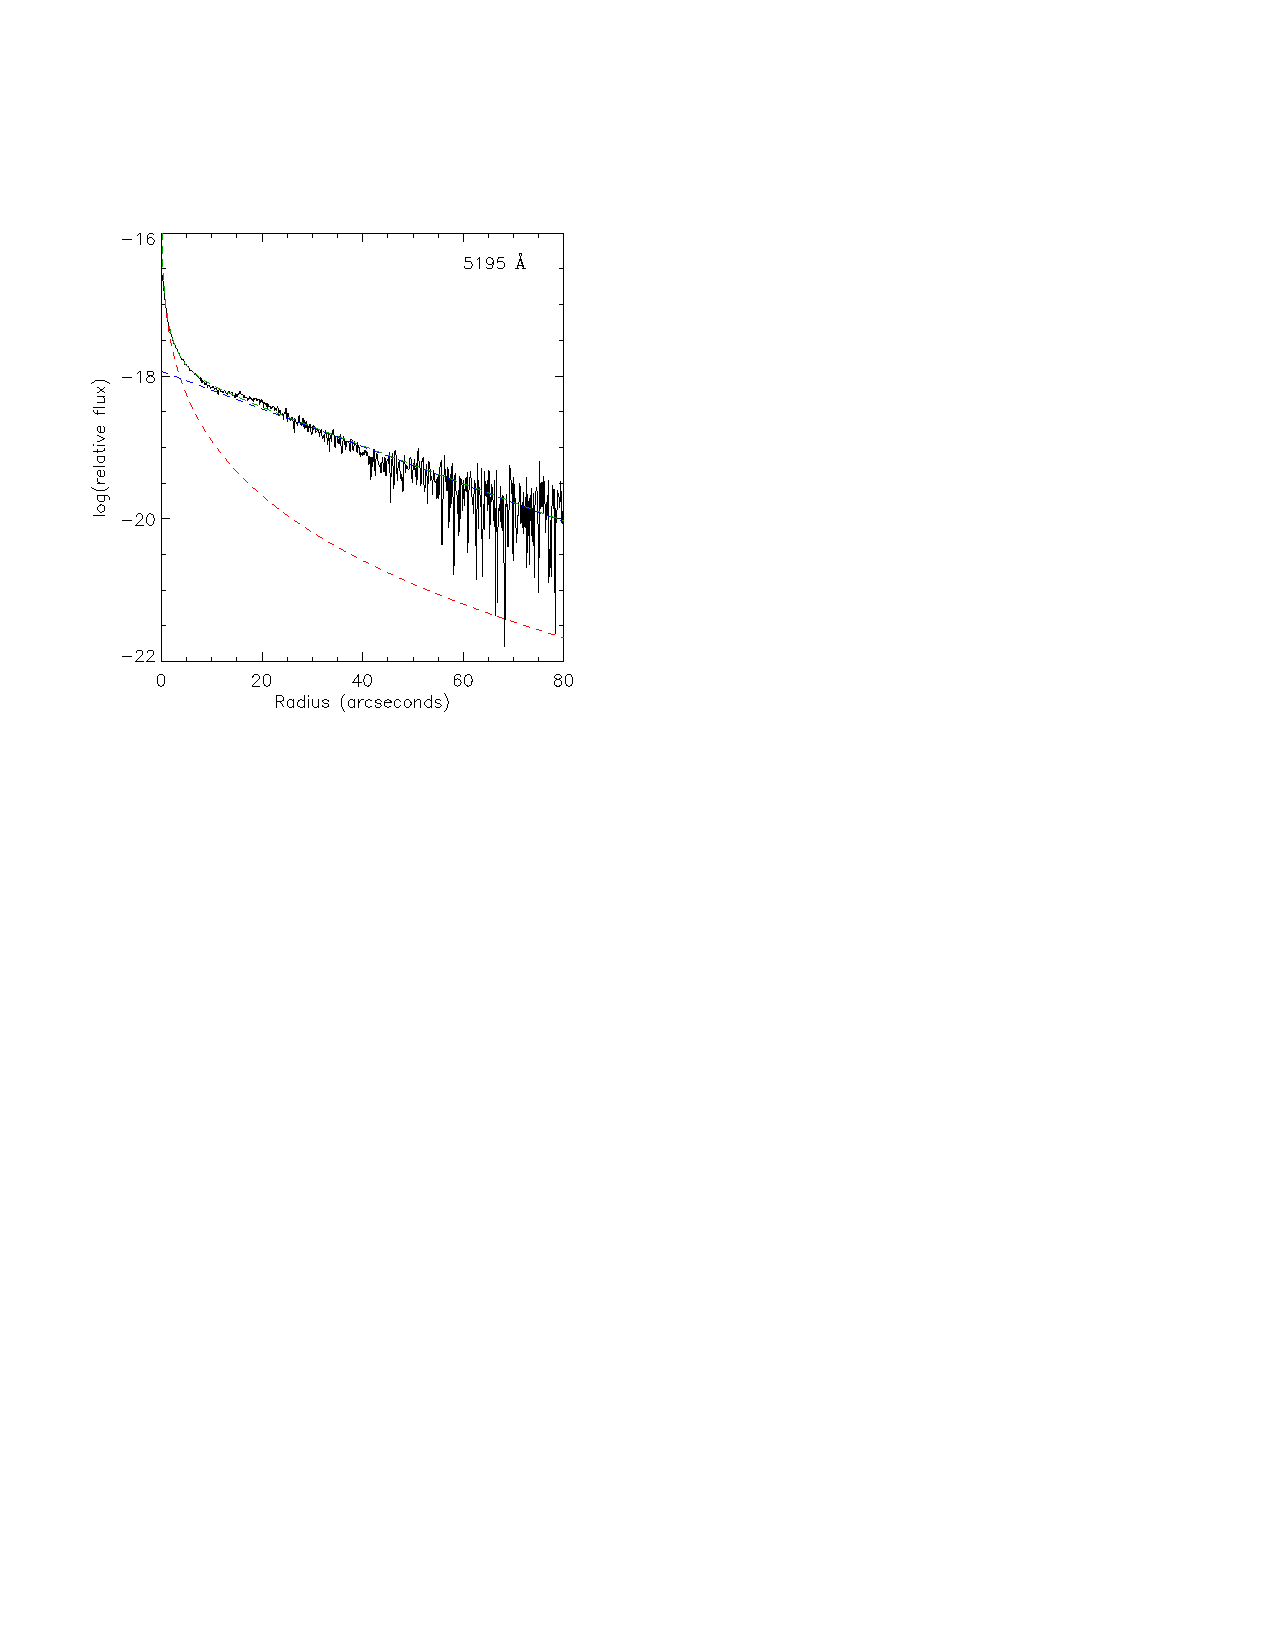
\includegraphics{figuras/johnston-decomp}
	\caption[Decomposição morfológica em uma dimensão] {Decomposição morfológica
	em uma dimensão. A linha preta mostra o perfil de brilho da galáxia NGC
	1375 em $5195\,\AA$. Em azul um perfil exponencial e em vermelho um
	perfil de De Vaucouleurs (Sérsic com $n=4$), que somados são o melhor
	ajuste, em verde. Retirado de \citet{Johnston2012}.}
	\label{fig:decompJohnston}
\end{figure}

Existem diversas ferramentas para fazer este ajuste de parâmetros. Vale citar,
por exemplo, GALFIT3 \citep{Peng2010}, BUDDA \citep{DeSouza2004}, GIM2D
\citep{Simard2002}, GASP2D \citep{MendezAbreu2008} e
Imfit\footnote{\url{http://www.mpe.mpg.de/~erwin/code/imfit/index.html}} por
Peter Erwin. Para o trabalho atual, o programa escolhido foi o Imfit, em grande
parte por ser de código livre, e também por estar escrito em C++, permitindo
trabalhar facilmente em Python. Como a versão original é um programa executado
em linha de comando, não é muito prático utilizá-la em seu formato original. Foi
feita uma versão ligeiramente
modificada\footnote{\url{https://github.com/streeto/Imfit}} do Imfit, em forma
de biblioteca compartilhada, para ser acessada por um programa escrito em
Python.


%***************************************************************%
%                                                               %
%               Decomposição: decomposicao espectral            %
%                                                               %
%***************************************************************%

\section{Decomposição espectral}

O artigo por \citet{Johnston2012} serviu como fonte de inspiração para este
trabalho. Nele, os autores obtém um espectro de fenda de galáxias lenticulares
(S0), tendo assim um perfil de brilho da galáxias para cada comprimento de onda.
Ajustando um perfil de Sérsic e um exponencial a cada um dos perfis (Figura
\ref{fig:decompJohnston}), eles obtém os espectros separados de cada um dos
componentes morfológicos (Figura \ref{fig:spectraJohnston}). 

\begin{figure}
	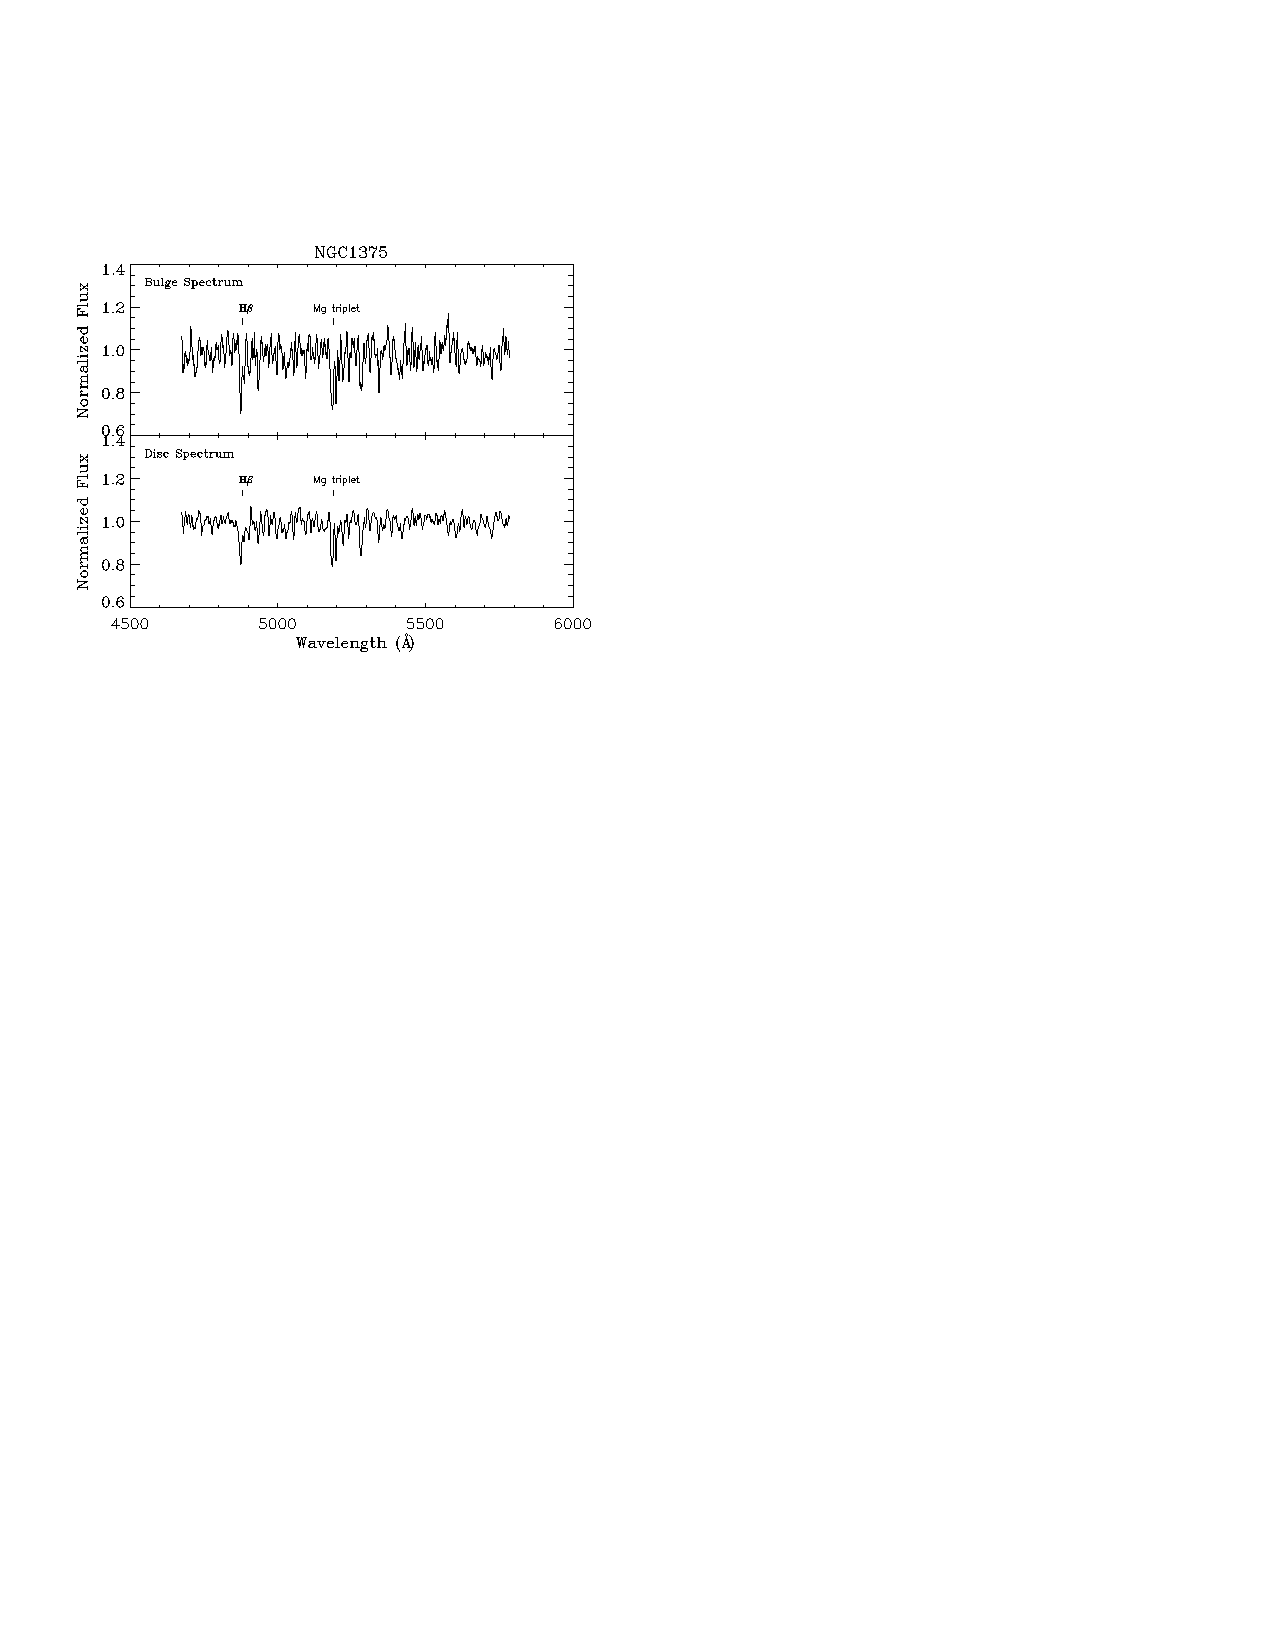
\includegraphics{figuras/johnston-spectra}
	\caption[Espectros das componentes morfológicas] {Espectros unidimensionais de
	disco e bojo de NGC 1375. Retirado de \citet{Johnston2012}.}
	\label{fig:spectraJohnston}
\end{figure}

O mesmo princípio foi então aplicado aos cubos de dados de IFS do CALIFA.
Diferente de do método de \citeauthor{Johnston2012}, foram ajustadas imagens a
cada comprimento de onda, utilizando um programa baseado na versão modificada do
Imfit, conforme a Seção \ref{sec:Decomp:decomp}. A decomposição é realizada
sobre os espectros sintéticos, provenientes de uma síntese realizada
anteriormente, sobre os dados originais. A motivação para isto é bastante
simples: evitar efeitos de linhas de emissão.
Estas seriam outra fonte de incerteza no ajuste morfológico, dado que em geral
estão relacionadas a regiões de formação estelar e núcleos ativos, que não
necessariamente seguem o mesmo perfil que o bojo ou o disco. Como este trabalho
é experimental, estas complicações foram deixadas de lado, neste momento.

Os resultados apresentados aqui devem ser tomados com cuidado. O ajuste é feito
sem fazer hipótese alguma sobre como os parâmetros morfológicos variam a cada
comprimento de onda. O projeto MegaMorph \citep{Haussler2013} está fazendo
essencialmente a mesma coisa: o ajuste morfológico dependente de comprimento de
onda de imagens de galáxia. A diferença é que no caso do MegaMorph utiliza-se
imagens de fotometria de banda larga do SDSS, e eles ajustam a variação dos
parâmetros morfológicos através de um polinômio \citep[Figura
\ref{fig:propertiesVika}]{Vika2013}. Aí se pode ver que em grande escala (em
comprimento de onda), há galáxias com um comportamento linear (ou até
razoavelmente constante) em $r_e$, porém outras apresentam variações mais
complexas. Este problema deve ser estudado mais a fundo futuramente neste
trabalho.

\begin{figure}
	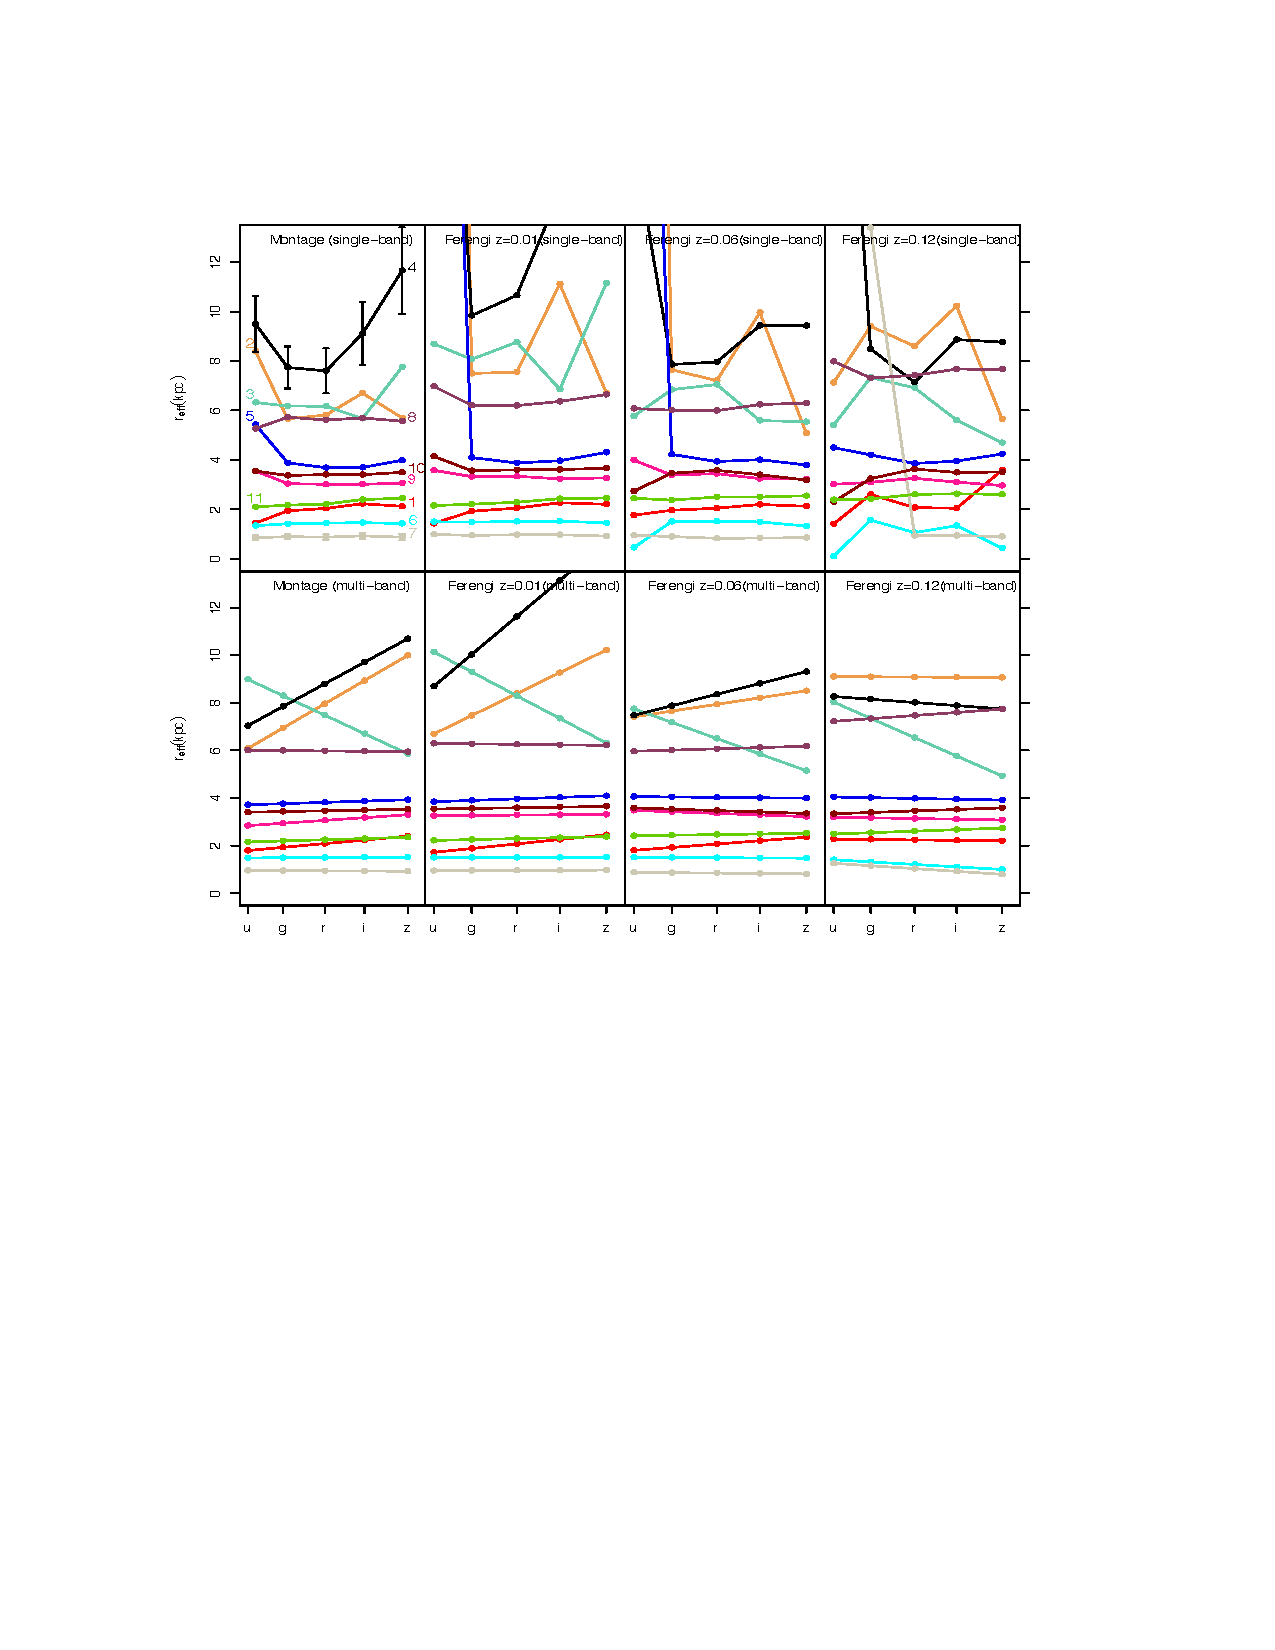
\includegraphics{figuras/vika-properties}
	\caption[Ajuste morfológico de bandas fotométricas] {Ajuste
	morfológico de 11 galáxias, utilizando as bandas fotométricas do
	SDSS. Os gráficos mostram o raio efetivo ($r_e$ neste trabalho) ajustado
	livremente a cada banda (painéis superiores), e com uma dependência linear em
	comprimento de onda (painéis inferiores). À esquerda estão os ajustes com as
	imagens originais, as colunas seguintes são para imagens com {\em redshift}
	artificiais. Retirado de \citet{Vika2013}.}
	\label{fig:propertiesVika}
\end{figure}

Para determinar se o método de decomposição funciona (ou melhor, se ele falha
mesmo para o caso mais básico), foi desenhado um exercício bastante simples.
Dado um conjunto de parâmetros morfológicos arbitrários, foi montado um cubo de
espectros de uma galáxia sintética composta de um bojo velho (utilizando uma SSP
de $12\,Gyr$) e um disco jovem (utilizando uma SSP de $3\,Gyr$). Os espectros de
base para o bojo e o disco podem ser vistos na Figura \ref{fig:testSpectra}.
Após gerar os cubos de dados de espectros, foi adicionado um ruído gaussiano de
$10\%$. Executando a decomposição neste cubo de dados simulado, deveria-se
encontrar valores para os parâmetros próximos aos escolhidos no início. A Figura
\ref{fig:testParameters} mostra a comparação dos parâmetros obtidos com os
iniciais. Os valores ajustados (linhas sólidas) estão de acordo com o valor
inicial, levando em conta o erro injetado nos espectros. É necessário repetir
este teste com configurações mais complexas, a fim de determinar as limitações
do método.


\begin{figure}
	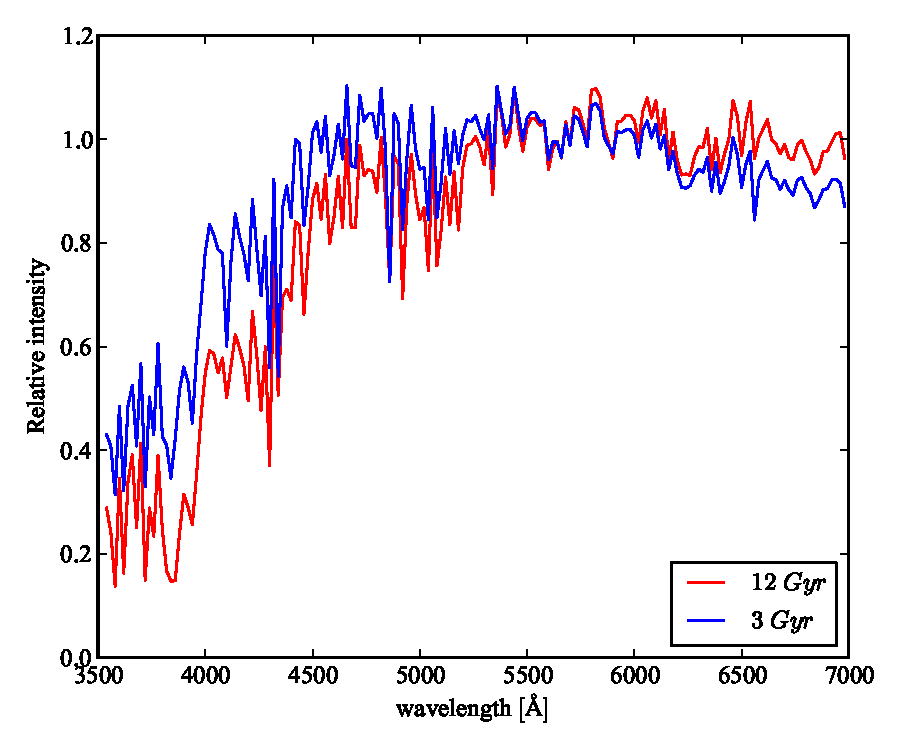
\includegraphics[width=0.7\columnwidth]{figuras/test-spectra}
	\caption[Espectros de base para o teste de decomposição] {Espectros de base
	para o teste de decomposição.}
	\label{fig:testSpectra}
\end{figure}


\begin{figure}
	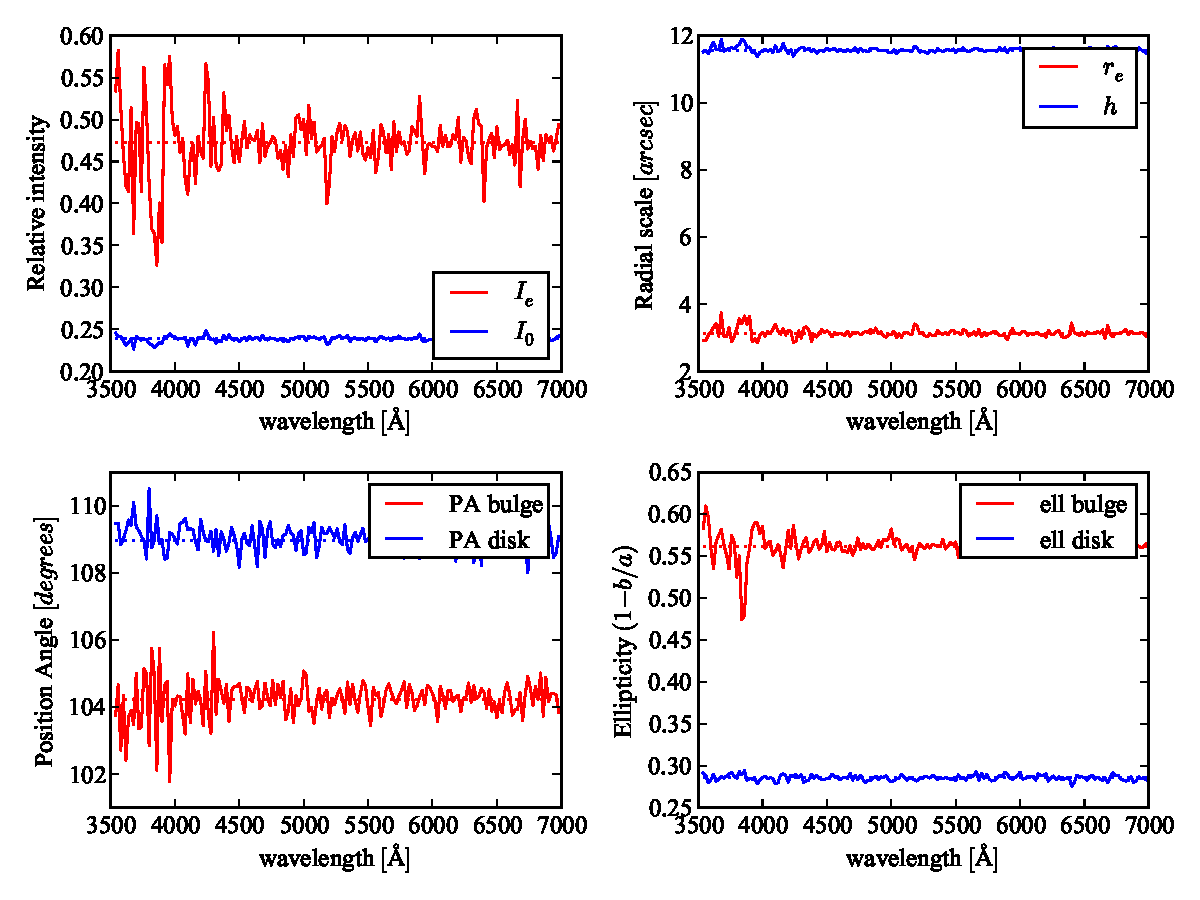
\includegraphics[width=1.0\columnwidth]{figuras/test-parameters}
	\caption[Parâmetros obtidos com o teste de decomposição] {Parâmetros obtidos
	com o teste de decomposição. Em tracejado são os parâmetros originais, em
	linhas sólidas os ajustes. Os parâmetros do bojo estão em vermelho e os do
	disco em azul. O índice de Sérsic ($n$) foi mantido constante e igual a $4$.}
	\label{fig:testParameters}
\end{figure}

A discussão a seguir refere-se à decomposição feita sobre os cubos de dados da
galáxia UGC 10695 (Figura \ref{fig:decompTarget}). A decomposição foi feita
utilizando a seguinte configuração:

\begin{figure}
	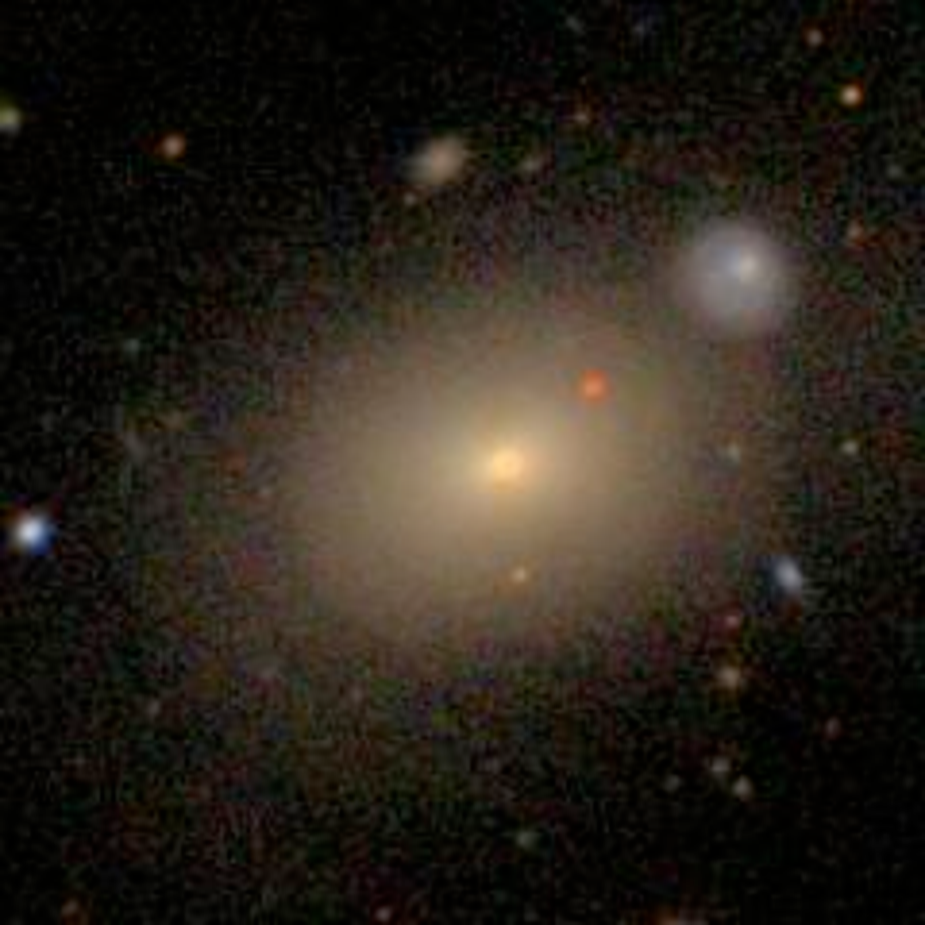
\includegraphics[width=0.3\columnwidth]{figuras/K0846}
	\caption[Montagem RGB da galáxia UGC 10695, do SDSS] {Montagem RGB da galáxia 
	UGC 10695, do SDSS.}
	\label{fig:decompTarget}
\end{figure}

\begin{itemize}

	\item Todos os pixels originais, sem agrupar em zonas de Voronoi.

	\item Espectros sintéticos provenientes de uma síntese executada anteriormente.

	\item Ajuste de todos os parâmetros livres: $I_e$, $r_e$, $n$, $I_0$, $h$ e a
	geometria da elipse\footnote{A geometria da elipse é definida pelo ângulo de
	posição ({\em P.A.}) e a elipticidade ($1 - b/a$).}.

	\item Convolução com uma PSF\footnote{{\em Point Spread Function}, a
	distribuição que representa a forma que uma fonte pontual aparece na imagem.}
	gaussiana de largura a meia altura de $2,4\,"$, medida numa estrela presente no
	campo observado.

\end{itemize}

Na Figura \ref{fig:decompParams} pode-se ver os parâmetros obtidos no ajuste
morfológico. Em comprimentos de onda menores que $4000\,\AA$ o ajuste sai um
pouco ruidoso, provavelmente devido à má calibração dos espectros do CALIFA
nesta região. Nas outras regiões os parâmetros tendem a variar suavemente,
embora haja variações locais próximas às linhas de absorção. Em especial, o
ângulo de posição do bojo e do disco, e o centro dos dois modelos, são
praticamente constantes.

A Figura \ref{fig:decompImages} permite uma visualização bidimensional dos
modelos em $5635\,\AA$, e uma comparação com a imagem original neste comprimento
de onda. O resíduo é mostrado no painel inferior direito. Ali se observa efeitos
de borda próximo às regiões externas mascaradas, além de um artefato no núcleo,
provavelmente devido à forma da PSF. Outra forma de visualizar a qualidade do
ajuste é através do perfil radial. A Figura \ref{fig:decompRadprof} mostra o
perfil radial em intervalos de aproximadamente $100\,\AA$. Ali se vê que o disco
e o bojo estão bem modelados, e que o ajuste é muito bom (o modelo é marcado com
uma linha preta pontilhada, e a sua maior parte fica sob a linha preta sólida, o
perfil original).

Os espectros obtidos são geralmente bem comportados. Um exemplo, a $5"$ do
núcleo, pode ser visto no painel superior da Figura \ref{fig:decompSpectra}.
O espectro de resíduo apresenta poucos artefatos. Nos painéis inferiores estão
os parâmetros de intensidade ($I_e$ e $I_0$) e de escala ($r_e$ e $h$), para
comparação.

\begin{figure}
	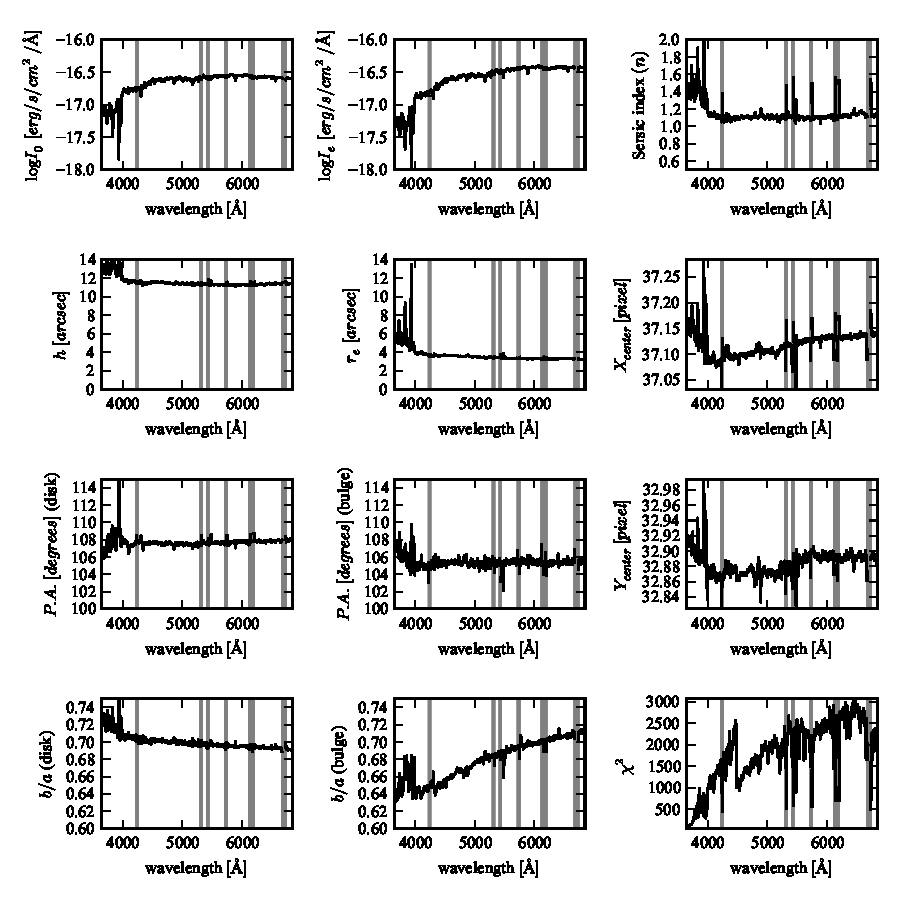
\includegraphics{figuras/decomp-fit-parameters}
	\caption[Parâmetros morfológicos] {Parâmetros morfológicos obtidos no ajuste
	de UGC 10695. Nos painéis à esquerda estão os parâmetros para o disco. Nos
	painéis ao centro, e no painel superior à direita, estãos os parâmetros do
	bojo. Ainda na coluna da direita há os painéis da posição do centro dos
	modelos e o $\chi^2$ do ajuste.}
	\label{fig:decompParams}
\end{figure}

\begin{figure}
	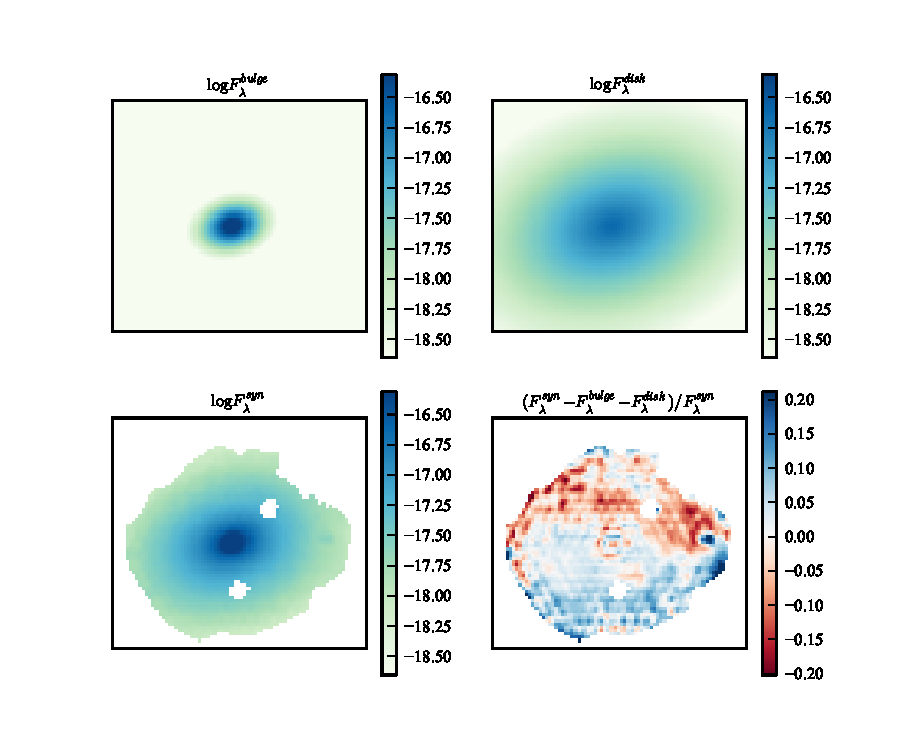
\includegraphics{figuras/decomp-model-images}
	\caption[Visualização 2-D da decomposição morfológica] {Visualização 2-D da
	decomposição morfológica. Nos painéis superiores os modelos de bojo e disco em
	$5635\,\AA$. No painel inferior à esquerda, a imagem original. No painel
	inferior à direita, o resíduo do ajuste, normalizado pela imagem original.}
	\label{fig:decompImages}
\end{figure}

\begin{figure}
	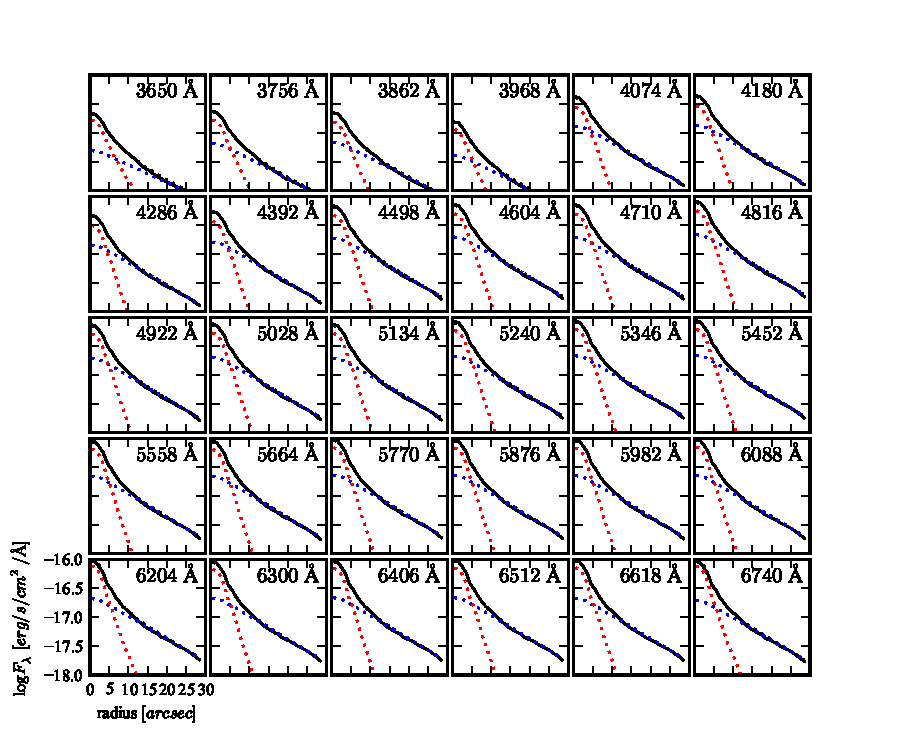
\includegraphics{figuras/decomp-radial-profile}
	\caption[Perfis radias da decomposição em função do comprimento de onda]
	{Perfis radias da decomposição em função do comprimento de onda.}
	\label{fig:decompRadprof}
\end{figure}

\begin{figure}
	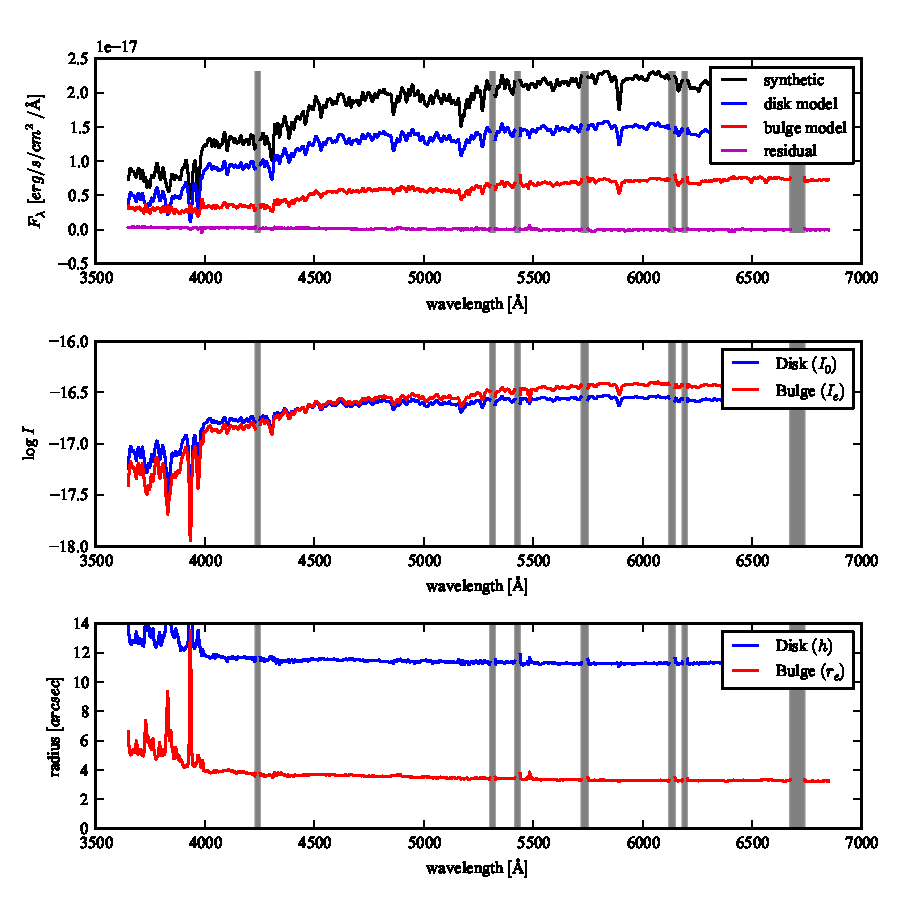
\includegraphics{figuras/decomp-model-quality}
	\caption[Espectro decomposto a $5"$ do núcleo] {Espectro decomposto a $5"$ do
	núcleo.}
	\label{fig:decompSpectra}
\end{figure}

Os cubos espectrais resultantes para bojo e disco foram passados pelo \starlight
como se fossem galáxias separadas, resultando em dois cubos de síntese extras
para a galáxia UGC 10695. O perfil radial de algumas propriedades físicas são
mostradas na Figura \ref{fig:decompSynRadprof}. O perfil de densidade
superficial de massa estelar é semelhante ao perfil de luminosidade, porém com
um bojo mais acentuado. Isto sugere um bojo velho (com maior razão
massa/luminosidade) e massivo. Como o bojo domina em luz e massa nas regiões
centrais, também é de se esperar que as propriedades pesadas por massa e luz
(idade e metalicidade) da galáxia original sejam mais próximas do valor do bojo
nesta região. O mesmo ocorre nas regiões externas, onde o disco domina, as
propriedades da galáxia refletem os valores do disco. Ou seja, o resultado é
consistente.
A interpretação do perfil radial de $A_V$ requer um pouco mais de cuidado. Em
geral se esperaria que o disco contivesse mais poeira do que o bojo.
Entretanto, uma inspeção visual na Figura \ref{fig:decompTarget} mostra
estruturas como anéis concêntricos, o que pode indicar que a galáxia está
sofrendo ou sofreu interação (a pequena galáxia a nordeste na imagem pode ser o
culpado). Neste caso é possível que a poeira não esteja distribuída como
normalmente se espera, mas isto é apenas especulação.

O histórico de formação estelar é mostrado na Figura \ref{fig:decompSynSfh}.
Aqui se vê um bojo (painel central) sendo formado por um surto de formação
estelar antigo e concentrado, com um episódio de formação estelar recente. Isto
é consistente com um cenário de interação. O disco se constrói de forma mais ou
menos uniforme até menos de $10^9$ anos atrás, porem não apresenta formação
estelar recente significativa na mesma época que o bojo.

\begin{figure}
	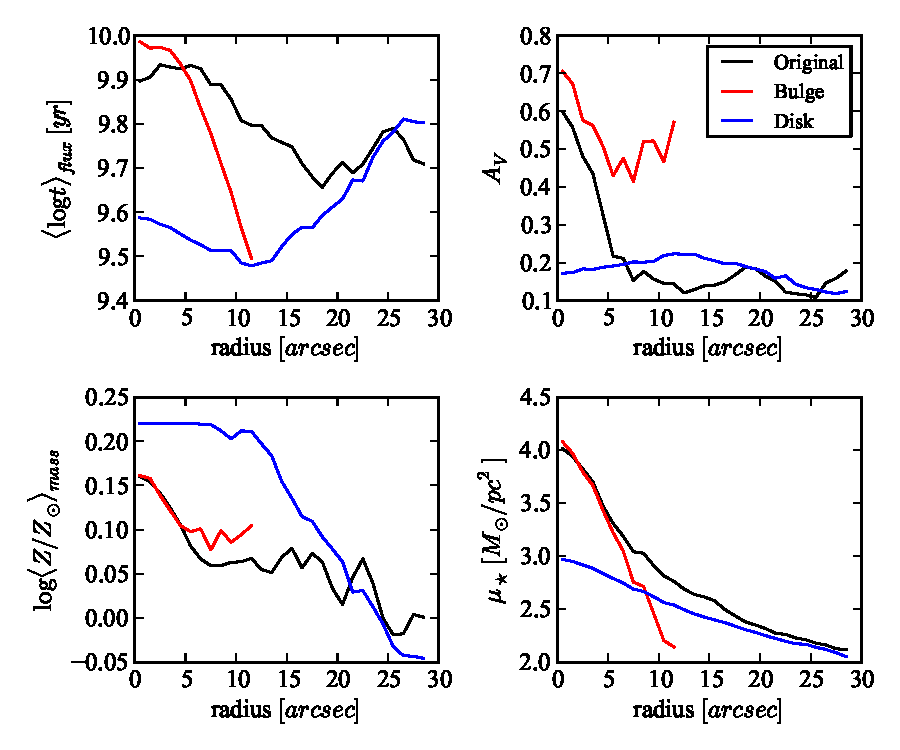
\includegraphics{figuras/decomp-at-aZ-AV-mu}
	\caption[Perfil radial das propriedades do bojo, disco, e total] {Perfil
	radial das propriedades físicas do bojo (vermelho), disco (azul), e original
	(preto). (cima, esquerda) Idade estelar média ponderada pela luminosidade.
	(baixo, esquerda) Metalicidade estelar média ponderada pela massa estelar.
	(cima, direita) Atenuação por poeira, na banda $V$. (baixo, direita) Desidade
	superficial de massa estelar. O Bojo vai somente até $12"$, que corresponde a
	$3\,R_{50}$.}
	\label{fig:decompSynRadprof}
\end{figure}

\begin{figure}
	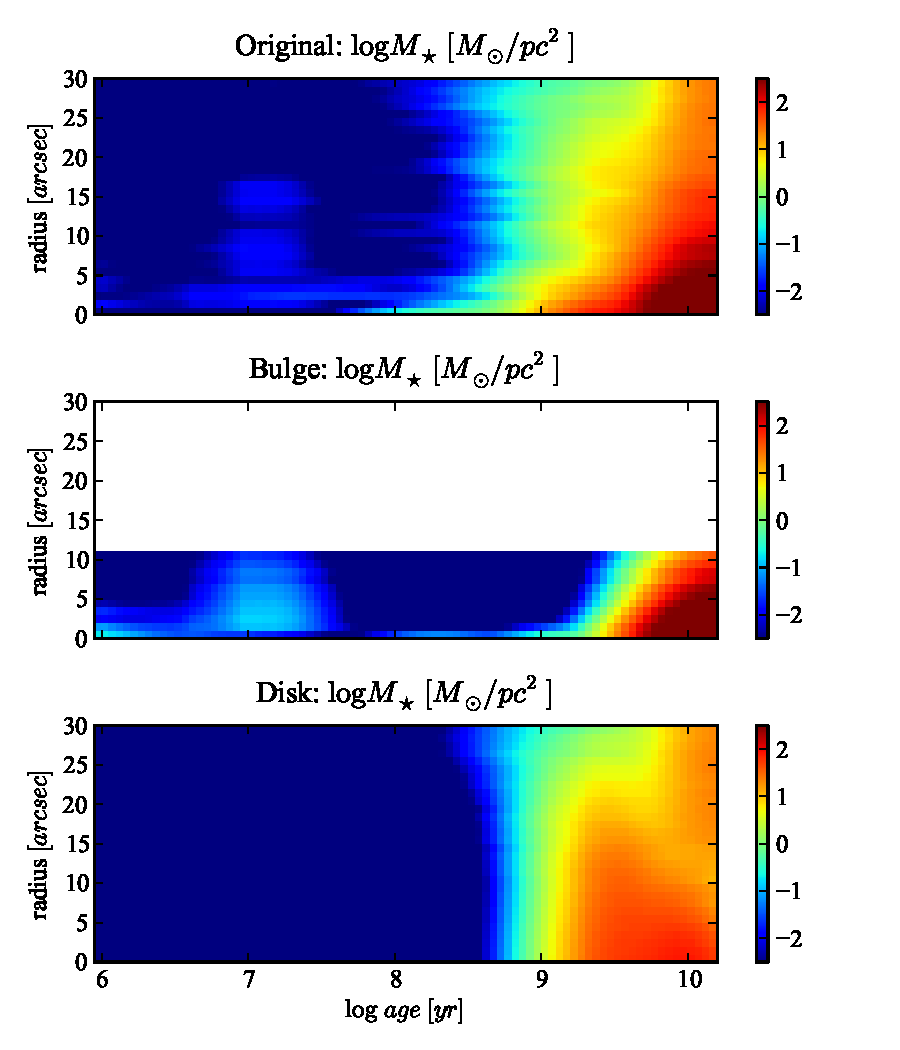
\includegraphics{figuras/decomp-sfh}
	\caption[Histórico de formação estelar do bojo, disco, e total] {Histórico de
	formação estelar da galáxia original (cima), bojo (meio) e disco (baixo). Os
	gráficos mostram quanta massa por unidade de área foi transformada em estrelas,
	em cada {\em bin} de raio e idade. O Bojo vai somente até $12"$, que
	corresponde a $3\,R_{50}$.}
	\label{fig:decompSynSfh}
\end{figure}

Através da decomposição morfológica realizada neste trabalho, foram obtidos
cubos de síntese espectral para o bojo e o disco de uma galáxia. As propriedades
físicas destas componentes são a grosso modo compatíveis com o que se espera de
um bojo e um disco. É preciso levar em conta, entretanto, que estes são resultados
preliminares. Testes similares aos apresentados anteriormente, com simulações de
galáxias com histórico de formação estelar mais realistas são fundamentais para
determinar a confiabilidade do método.


%% End of this chapter
